\documentclass[a4paper,10pt]{article}
\usepackage[utf8x]{inputenc}
\usepackage{graphicx}

%opening
\title{Assignement 2}
\author{Shuying Dong, Roman Karlstetter}

\begin{document}



\section{Shared-Memory $\pi$-Berechnung}
The sum has to be multiplied by $4\cdot h$, because
\begin{itemize}
 \item every element has to be multiplied by $h$ (according to Mittelpunktsregel) and
 \item $arctan(1) = \frac{\pi}{4}$ ($arctan$ is $tan^{-1}$ and $tan(\frac{\pi}{4}) = tan(45°) = 1$), so it holds that: $\pi = 4 \cdot arctan(1)$. 
\end{itemize}

Interestingly, we don't get the same result for all three methods. The reason for this are probably rounding errors. 

Forthermore, for the openmp-reduction and the sequential version, we always get the same result, for the critical section version, we always get different results. This shows, that the order in which the different parts of the integral are summed up is not defined and so, in every run of the programm, we get different rounding errors.

\paragraph{Runtime}
\begin{itemize}
 \item[Sequencial] not so surprising, we always get approximately the same runtime.
 \item[Critical Section] if we increment the number of threads, the runtime goes up dramatically. The reason for this is probably the locking which has to be done in order to guarantee exclusive access in the critical section. Even with only one thread it is slower for the same reason (locking).
 \item[Reduction Clause] for this, we get good scaling behaviour up to 8 threads, after that the performance decreases again and more or less stays at the same level. See the images for further details.
\end{itemize}

When using critical sections, the runtime goes up:
\begin{center}
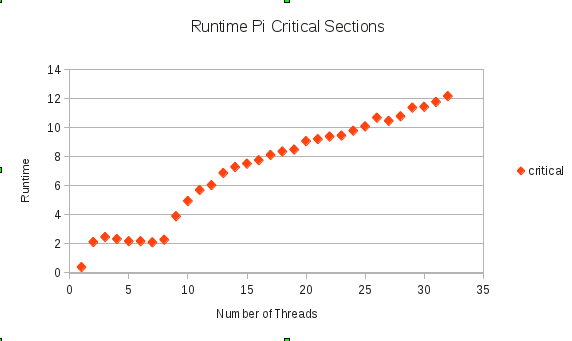
\includegraphics[]{pi_critical.png}
\end{center}
If reduction is used, if goes down:
\begin{center}
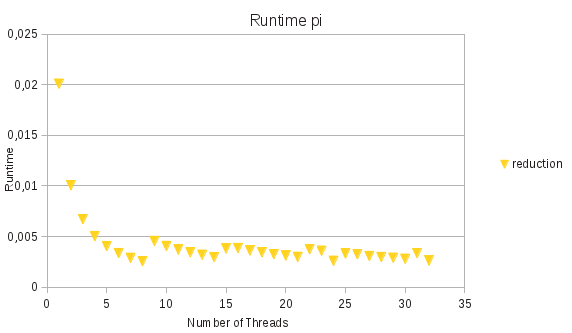
\includegraphics[]{pi_reduction.png}
\end{center}

\begin{center}
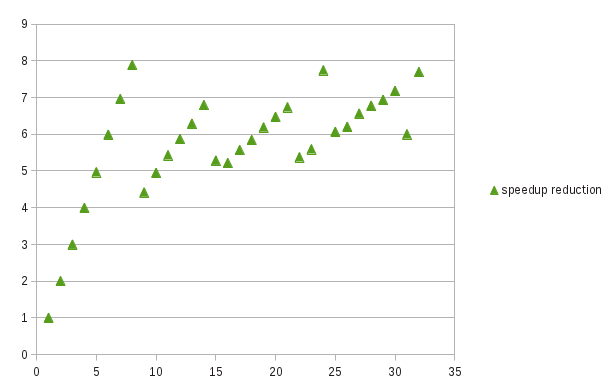
\includegraphics[]{pi_speedup.png}
\end{center}
\begin{center}
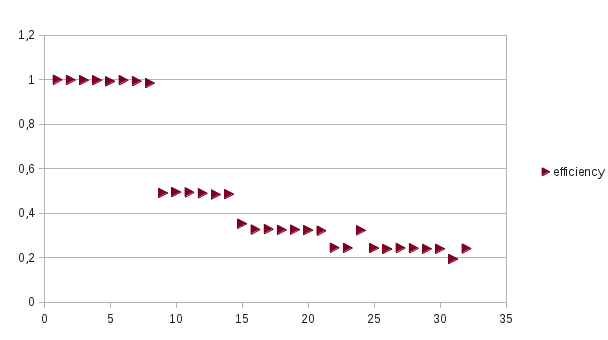
\includegraphics[]{pi_efficiency.png}
\end{center}
We use 8 cores for our measurements.

\section{Matrix-Matrix-Multiplikation II}

\section{Quicksort}
\begin{center}
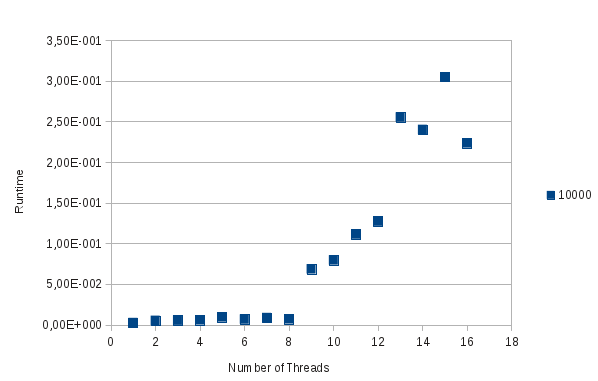
\includegraphics{strong_scaling_10000.png}\\
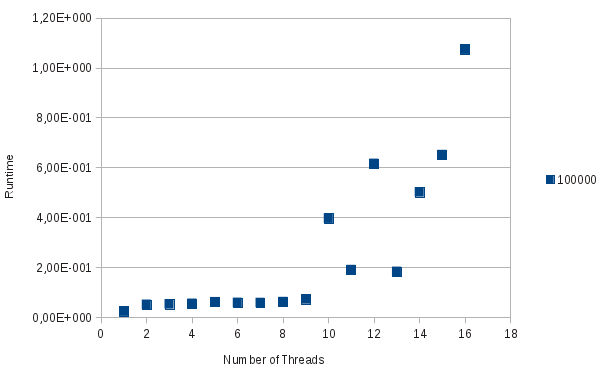
\includegraphics{strong_scaling_100000.png}\\
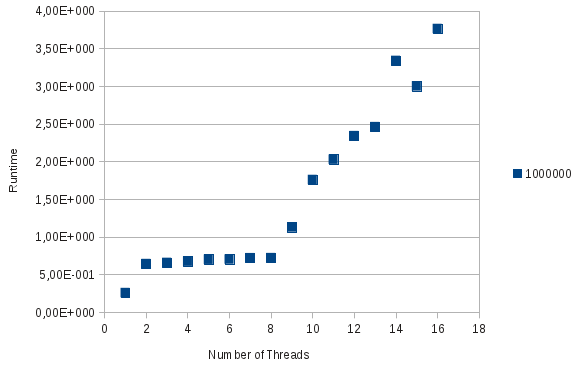
\includegraphics{strong_scaling_1000000.png}\\
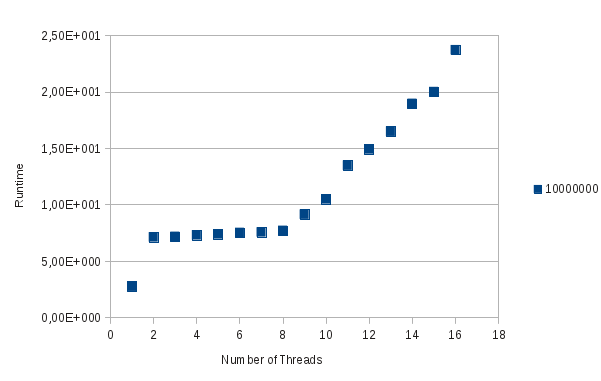
\includegraphics{strong_scaling_10000000.png}\\
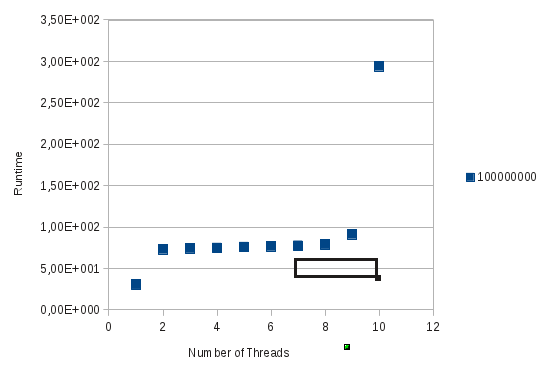
\includegraphics{strong_scaling_100000000.png}\\\end{center}

\end{document}
